\section{Hardware Architecture}
\label{sec:hardware}
\subsection{Overview}
Each GPU contains several multiprocessors (current hardware up to 
In contrast to the more sequential CPU computational flow, GPUs work highly parallelized.

This parallelization is because of many more computational cores 

Due to GPU hardware having more cores than CPUs, computation is organized into threads which are meant to be executed in parallel, grouped into multiple \textbf{blocks}, called a \textbf{grid}. Both grids and threadblocks can have a dimension up to 3. Using these constructs, it is easily possible to index a multidimensional structure.\\
Grids are created upon a call of a \textbf{kernel} - that is a code sequence running on CUDA-capable devices - (?). Below is an illustrated overview of one two dimensional grid (3x3) of blocks each running a number of threads.\\
\begin{figure}
    \centering
    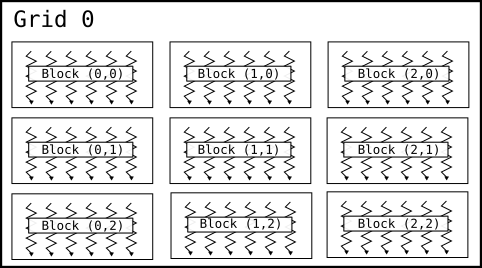
\includegraphics[scale=0.5]{media/threads_blocks_grid.png}
\end{figure}
\\
CUDA assigns blocks to streaming multiprocessors, 
\subsection{Memory}
\subsubsection{Device}
\paragraph{Global Memory}
\label{hardware_global}
The most ample of all GPU memory, often exceeding several gigabytes on current hardware, is accessible to all threads on the GPU and per PCIe even to the host.\\
Global memory is located off-chip, resulting in a higher latency around 500 clock cycles which is often hidden through thread parallelism but still a way higher bandwidth than the connection per PCI Express between host and device.\\
Memory transactions are used to global memory and these have to be aligned to their transaction size of 32, 64 or 128 bytes.\\
The high latency can impose a significant performance loss, to minimize its impact CUDA will try to merge as many transactions as possible. We will explore these coalescing mechanisms later in ~\ref{global_access}.\\
\paragraph{Shared Memory}
Due to being located on-chip, therefore resulting in low-latency, high-bandwidth memory, shared memory is used to exchange data between threads in a block and synchronize them.\\
Additionally shared memory is ideally suited to manually cache global memory.\\
\paragraph{Registers}
Data used without keywords (shared, global aka device) in a kernel are stored in registers, as long as they can hold it.\\
Though there are multiple thousands register (between 32K and 128K for current hardware) available for use by the compiler,
these registers have to be split between concurrently running threads on a multiprocessor.\\
Should the compiler decide that local data is too big to be hold in register only,
it will be stored in local memory which is by orders slower than registers or shared memory.\\
This phenomenon is called \emph{register pressure} and should be avoided by investigating local memory usage
and using shared memory.\\
\paragraph{Local Memory}
Contrary to its name is local memory not located on-chip, but in global memory.
Therefore it inherits its characteristics, most important the high latency which may limit an applications performance immensly.
To avoid local memory usage, the compiler supports a switch called \emph{--ptxas-options=-v} with which several information regarding
the generated code is shown. 
\paragraph{L1 Cache}
L1 Cache is on-chip memory, caching access to local memory. Shared memory and L1 cache are sharing the same memory space. \\
\paragraph{L2 Cache}
In contrast to L1 cache, L2 Cache is shared between all multiprocessors and is used to cache access to local and global memory.\\
% TODO: show when introduced etc.
\paragraph{Texture Memory \& Cache}
Texture memory can be used to hold data aswell and is optimized to store two dimensional data.\\
\subsubsection{Transfer}
GPUs are connected to a hostsystem via PCI Express, which limits the bandwidth of the memory transfer between host and device.\\
PCI Express is a point-to-point system (source?) and as data exchange is done using packets,
there is a significant overhead involved.\\
\begin{table*}
\centering
\begin{tabular}{c|c|c|c}
\textbf{Generation} &   \textbf{Transfer-Rate}      & \textbf{per Lane} & \textbf{16-lane}\\
\hline\hline
PCIe 1.0     &   2.5 GT/s               & 2 GBit/s          & 32 Gbit/s\\
PCIe 2.0     &   5.0 GT/s               & 4 GBit/s          & 64 GBit/s\\
PCIe 3.0     &   8.0 GT/s               & 7.87 GBit/s       & 126 Gbit/s\\
PCIe 4.0     &   16.0 GT/s              & 15.754 GBit/s     & 252 GBit/s\\
\hline
\end{tabular}
\caption{Comparison of different iterations of the PCI Express protocol, source: pcisig.com}
\label{tab:pci_comp}
\end{table*}
\emph{**show GPU Global memory transfer rates**}
As a comparision, GDDR5 (double rate type 5 synchronous graphics random access memory) is able to maintain a bandwith in excess over 100/200 GB/s.
\\
As we can see, the GPU memory is several times faster than the PCIe protocol theoretical maximum bandwidth.\\
This means we will have to try to minimize data transfer between host and device as PCIe is many times slower than device memory.
We will exploit this knowledge to achieve (?) high computational throughput (?).
\subsection{Kernel}
A \emph{Kernel} is a code procedure launched from the host and executed in a grid of threadblocks on the graphics unit.\\
Once the CUDA code is loaded onto the GPU, a global scheduler distributes the threadblocks to the streaming processors, in which then warp schedulers select 32 threads ( one warp ) for execution.\\
